%%%%%%%%%%%%%%%%%%%%%%%%%%%%%%%%%%%%%%%%%%%%%%%%%%%%%%%%%%%%%%%%%%%%%%%%%%%%%%%%
%2345678901234567890123456789012345678901234567890123456789012345678901234567890
%        1         2         3         4         5         6         7         8

\documentclass[letterpaper, 10 pt, conference]{ieeeconf}  % Comment this line out if you need a4paper

%\documentclass[a4paper, 10pt, conference]{ieeeconf}      % Use this line for a4 paper

\IEEEoverridecommandlockouts                              % This command is only needed if 
                                                          % you want to use the \thanks command

\overrideIEEEmargins                                      % Needed to meet printer requirements.

% See the \addtolength command later in the file to balance the column lengths
% on the last page of the document

% The following packages can be found on http:\\www.ctan.org
%\usepackage{graphics} % for pdf, bitmapped graphics files
%\usepackage{epsfig} % for postscript graphics files
%\usepackage{mathptmx} % assumes new font selection scheme installed
%\usepackage{times} % assumes new font selection scheme installed
%\usepackage{amsmath} % assumes amsmath package installed
%\usepackage{amssymb}  % assumes amsmath package installed
\usepackage{graphicx}
\usepackage[export]{adjustbox}
\usepackage{hyperref}
\graphicspath{ {images/} }


\title{\LARGE \bf
Multi-robot Patrolling with Duckiebots
}


\author{Pin-Wei Chen$^{1}$% <-this % stops a space
\thanks{*This work was supported by the Robotics Master Program in National Chiao Tung University, Taiwan}% <-this % stops a space
\thanks{$^{1}$Pin-Wei Chen, National Chiao Tung University, Taiwan.		{\tt\small ccpwearth@gmail.com}}%
}


\begin{document}



\maketitle
\thispagestyle{empty}
\pagestyle{empty}


\section{INTRODUCTION \& MOTIVATION}

Multi-robot patrolling is an potential idea, I can apply this project to surveillance, security, production line, etc. I realize that robot can help us with something routine and cycling, such as patrolling, which I should patroll lots of nodes again and again. As a result, I come up with this idea, trying to build a multi-robot patrolling system in ROS, and also combine this system with duckietown.

\section{SYSTEM ARCHITECTURE \& EQUIPMENTS}

\subsection{SYSTEM ARCHITECTURE}

We will have lots of robots(duckiebots) and one master robot(Raspberry Pi3). The all robots and master are all connected to the same router, so that the master can communicate with each robot.

Each robot will follow the yellow line, and when they arrive at the patrolling node, they will stop and wait for the order from the master. The master will tell the robot to keep go forward or turn back as each robot arrived at the patrol node.

\subsection{EQUIPMENTS} 

The robot I use is Moified from duckiebot, I replace the dagu motor with JGB37-520 motor which have an encoder in it Fig.~\ref{figure:JGB37-520}. In addition, I use yellow lines and black background as our patrol map, and I use apriltags as the patroll nodes Fig.~\ref{figure:map}. In software part, I use ROS kinetic and ubuntu 16.04 LTS as my develop enviromnet.

\begin{figure}[h] % h means put this image here
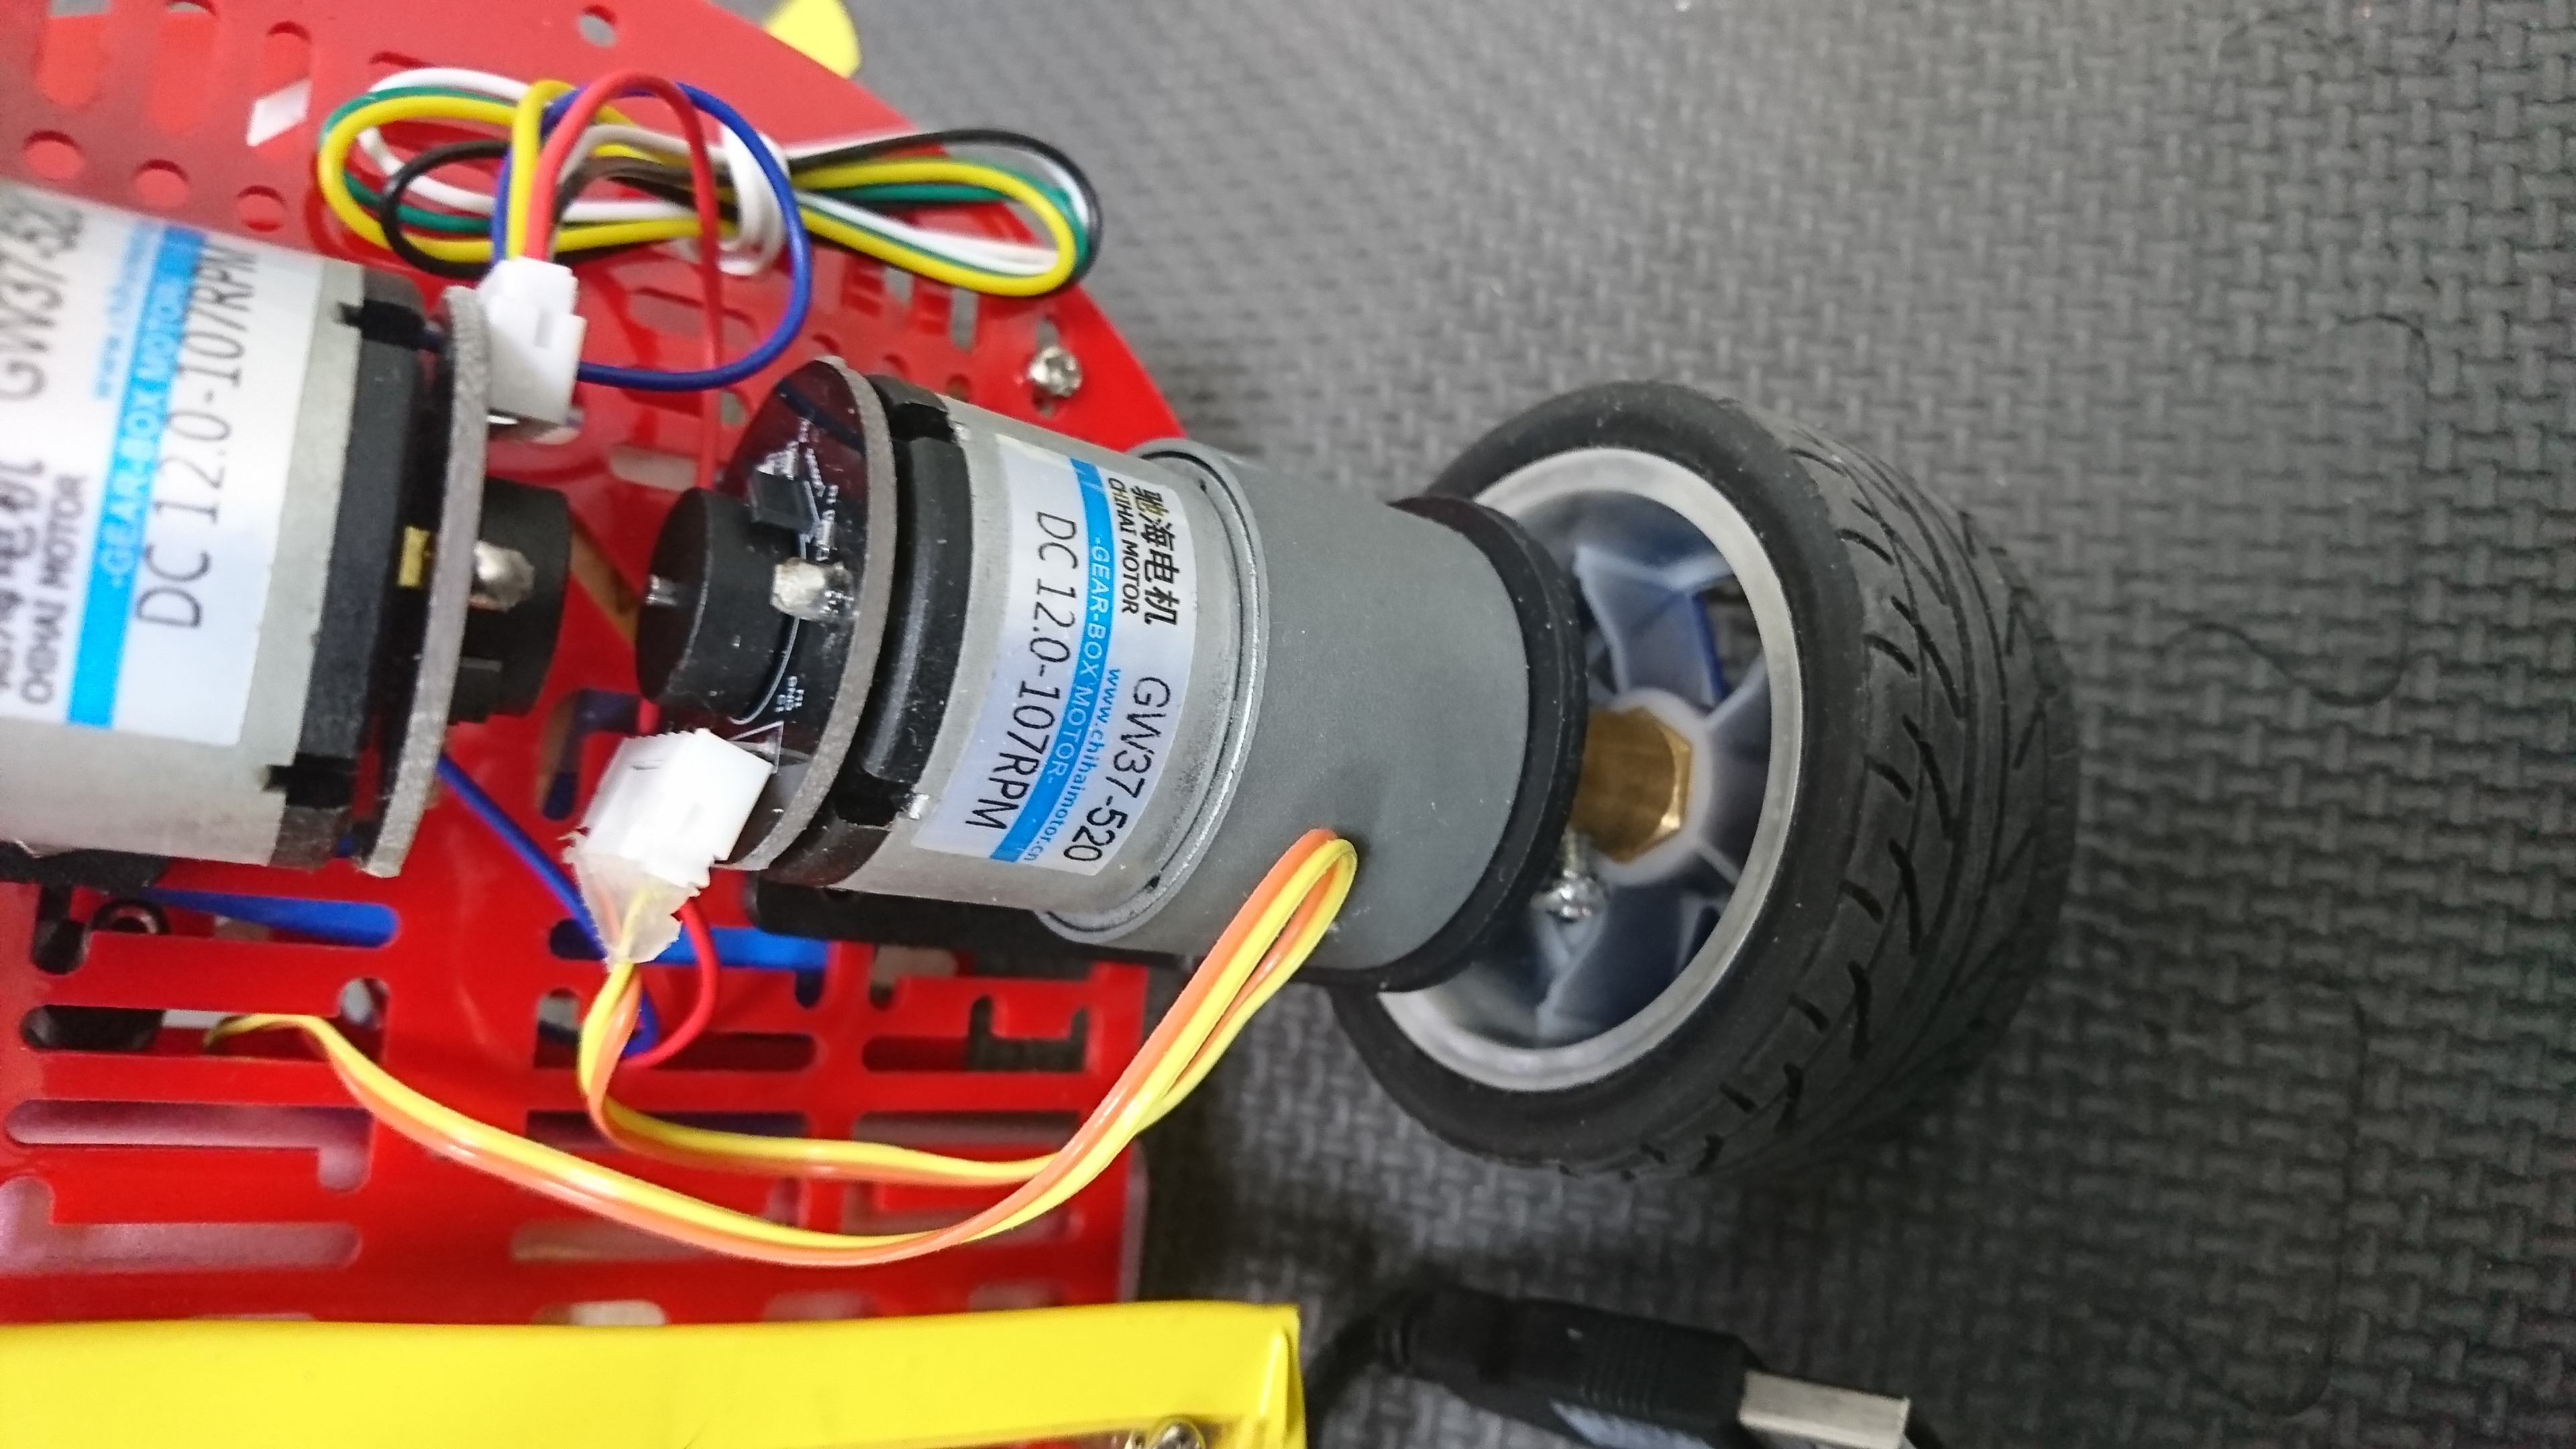
\includegraphics[width=0.8\columnwidth]{JGB37-520}
\centering
\caption{JGB37-520 encoder motor}
 \label{figure:JGB37-520}
\end{figure}

\begin{figure}[t] % t means put this image at the top 
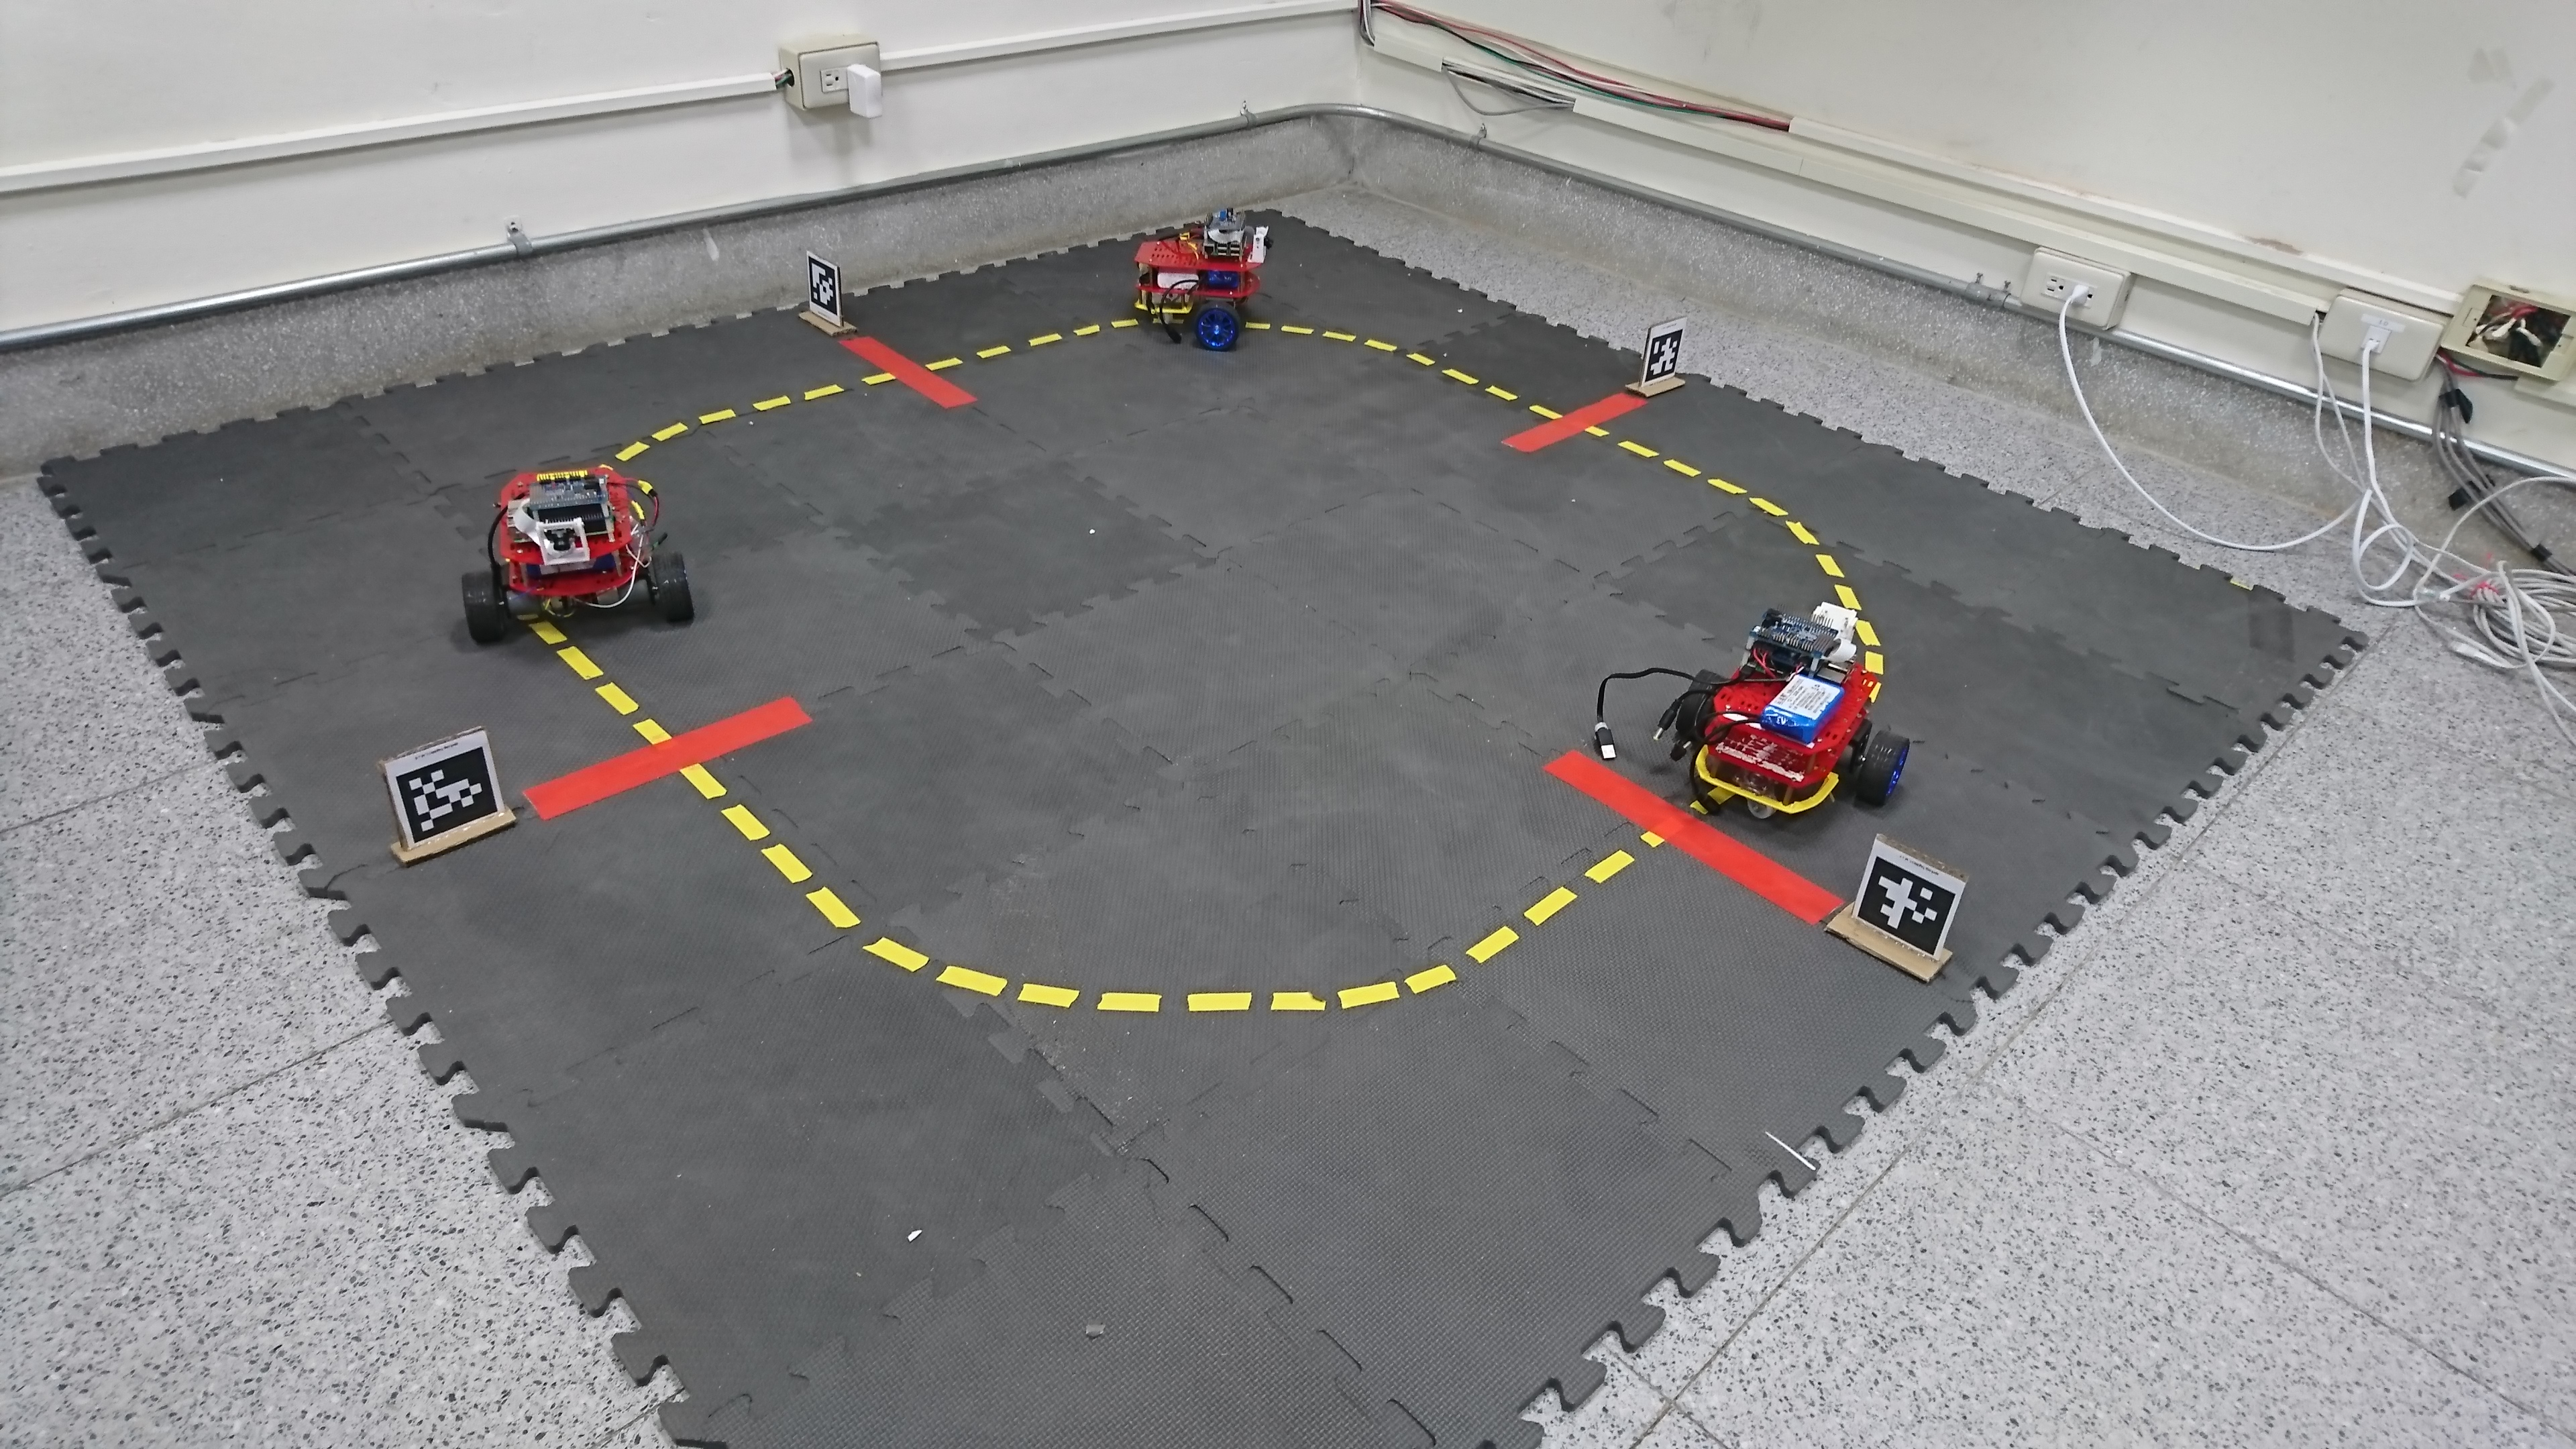
\includegraphics[width=0.8\columnwidth]{map}
\centering
\caption{Multi-robot patrolling map}
\label{figure:map}
\end{figure}

\section{SPECIFIC AIMS}

\begin{itemize}
\item Real world patrolling system
\end{itemize}
I am trying to let multi-robot follow the yellow line and patrol multi-node(apriltags), so that each node will be patolled in approximately the same idle time. Moreover, those robot will not patol on the same lane at the same time, or they will crash with each other.
\begin{itemize}
\item Virtual world patrolling system
\end{itemize}
I will build a virtual world and models in Gazebo, and try to move all of my patrolling system to Gazebo, so that we can easily show the concept of patrolling robot in virtual world. Moreover, we can connect real world and gazebo, so that it will easily enable us to show the status of each robot and node in gazebo.

\section{APPROACH}

I will modify the lane following in duckietown, to let my robot can patrol along the yellow line. And I will use apriltags with different ID to let the robot know which node they are patrolling now, it's kind of locate the robot.

The algorithm I use is refer to "Distributed On-line Dynamic Task Assignment for Multi-robot Patrolling"~\cite{Farinelli:2017:DOD:3124264.3124274}, we will measure the idleness of each node first, and than the master robot will coordinate every robot to let the nodes with large idleness be patrolled first. If any node is going to be patrolled, the idleness will return to zero, so that no two robots will go to the same node at the same time, and it can avoid collision.   


\section{SCHEDULE AND TEAM COLLABORATION}

I expect this project can finish real world patrolling before November, and can excute in Gazebo before December. And the experiment video is available in this link: \url{https://goo.gl/sDwa9j}

\addtolength{\textheight}{-12cm}   % This command serves to balance the column lengths
                                  % on the last page of the document manually. It shortens
                                  % the textheight of the last page by a suitable amount.
                                  % This command does not take effect until the next page
                                  % so it should come on the page before the last. Make
                                  % sure that you do not shorten the textheight too much.

\bibliographystyle{IEEEtran}
\bibliography{egbib}

\end{document}
